\documentclass[tikz, border=2pt]{standalone}
\usepackage{tikz}
\begin{document}
    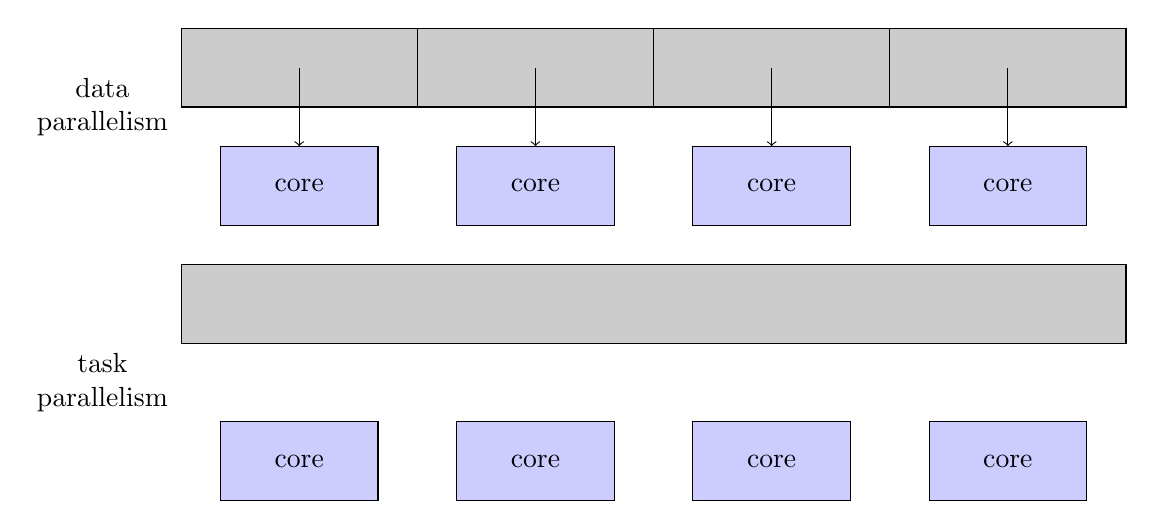
\begin{tikzpicture}
        \draw [fill=black!20] (0,2) rectangle (12,3);
        \foreach \x in {0,3,6,9}
        {
            \draw [fill=black!20] (\x, 5) rectangle (\x+3,6);
            \draw [->] (\x+1.5, 5.5) -- (\x+1.5, 4.5);
            \draw [fill=blue!20] (\x+0.5,3.5) rectangle (\x+2.5,4.5);
    \draw [fill=blue!20] (\x+0.5,1) rectangle (\x+2.5,0);
        }
        \foreach \x in {0.5,...,3.5}
        {
            \node at (\x*3, 4) {core};
            \node at (\x*3, 0.5) {core};
        }
        \node [align=center] at (-1, 5) {data\\parallelism};
        \node [align=center] at (-1, 1.5) {task\\parallelism};
    \end{tikzpicture}
\end{document}